\documentclass[12pt,a4paper,reqno]{amsart}

% section handling
\usepackage{subfiles} 

% language
\usepackage[greek,english]{babel}
\usepackage[utf8]{inputenc}
\usepackage{alphabeta}

% change default names to greek
\addto\captionsenglish{
    \renewcommand{\contentsname}{Περιεχόμενα}
    \renewcommand{\refname}{Βιβλιογραφία}
    \renewcommand{\datename}{Ημερομηνία:}
    \renewcommand{\urladdrname}{Ιστοσελίδα}
}

% math 
\usepackage{amsmath,amsthm,amssymb,amscd}

% font
\usepackage[cal=euler]{mathalfa}
\usepackage{libertinus-type1}
% \usepackage{txfonts} % for upright greek letters
\usepackage{bm} % for bold symbols
\usepackage{bbm} % for the simply-looking bb symbols

% miscellaneous 
\usepackage{changepage} %for indenting environments
\usepackage{csquotes} % example: \textcquote{}

% drawing
\usepackage{tikz,tikz-cd}
\usetikzlibrary{shapes.misc, patterns, matrix, calc, intersections,positioning}
\usepackage{graphics,graphicx}
\usepackage{float} % provides enhanced control and customization options for floating objects such as figures and tables

% colors
\usepackage{xcolor}
\definecolor{darkcandyapplered}{rgb}{0.64, 0.0, 0.0}
\definecolor{midnightblue}{rgb}{0.1, 0.1, 0.44}
\definecolor{mylightblue}{HTML}{336699}

% hrefs
\usepackage{hyperref}
\usepackage[noabbrev,capitalize]{cleveref}
\hypersetup{
    pdftoolbar=true,        
    pdfmenubar=true,        
    pdffitwindow=false,     
    pdfstartview={FitH},  % fits the width of the page to the window
    pdftitle={},
    pdfauthor={},
    pdfsubject={},
    pdfkeywords={},
    pdfnewwindow=true,  % links in new window
    colorlinks=true,  % false: boxed links; true: colored links
    linkcolor=darkcandyapplered,   % color of internal links
    citecolor=midnightblue,  % color of links to bibliography
    urlcolor=cyan,  % color of external links
    linktocpage=true  % changes the links from the section body to the page number
    }

% geometry
\textwidth=16cm 
\textheight=21cm 
\hoffset=-55pt 
\footskip=25pt

% thm envs (you might need to change the path)
% In this macro I define all the theorem environments

\theoremstyle{definition}
\newtheorem{theorem}{Θεώρημα}
\newtheorem{proposition}[theorem]{Πρόταση}
\newtheorem{lemma}[theorem]{Λήμμα}
\newtheorem{corollary}[theorem]{Πόρισμα}
\newtheorem{conjecture}[theorem]{Εικασία}
\newtheorem{problem}[theorem]{Πρόβλημα}
\newtheorem*{claim}{Ισχυρισμός}
\newtheorem{observation}[theorem]{Παρατήρηση}
\newtheorem{definition}[theorem]{Ορισμός}
\newtheorem{question}[theorem]{Ερώτηση}
\newtheorem{example}[theorem]{Παράδειγμα}
\newtheorem{exercise}{Άσκηση}

\theoremstyle{remark}
\newtheorem*{remark}{Παρατήρηση}

% fixes the correct numbering of environments
\numberwithin{theorem}{section}
\numberwithin{exercise}{section}
\numberwithin{equation}{section}

% math ops (you might need to change the path)
% In this macro I define all of my math operators

% fields
\newcommand{\NN}{\mathbbmss{N}} 
\newcommand{\ZZ}{\mathbbmss{Z}} 
\newcommand{\QQ}{\mathbbmss{Q}} 
\newcommand{\RR}{\mathbbmss{R}} 
\newcommand{\CC}{\mathbbmss{C}} 
\newcommand{\KK}{\mathbbmss{K}} 
\newcommand{\FF}{\mathbbmss{F}} 

% symmetric group
\newcommand{\fS}{\mathfrak{S}}  

% calligraphic 
\newcommand{\aA}{\mathcal{A}} 
\newcommand{\bB}{\mathcal{B}}
\newcommand{\cC}{\mathcal{C}}
\newcommand{\dD}{\mathcal{D}}
\newcommand{\eE}{\mathcal{E}}
\newcommand{\fF}{\mathcal{F}}
\newcommand{\hH}{\mathcal{H}}
\newcommand{\iI}{\mathcal{I}}
\newcommand{\lL}{\mathcal{L}}
\newcommand{\oO}{\mathcal{O}}
\newcommand{\pP}{\mathcal{P}}
\newcommand{\sS}{\mathcal{S}}
\newcommand{\mM}{\mathcal{M}}
\newcommand{\uU}{\mathcal{U}}

% bold
\newcommand{\bfa}{\mathbf{a}}
\newcommand{\bfe}{\mathbf{e}}
\newcommand{\bfF}{\pmb{F}}
\newcommand{\bfR}{\pmb{R}}
\newcommand{\bfv}{\mathbf{v}}
%\newcommand{\bfx}{\bm{x}}
%\newcommand{\bfx}{\mathbf{x}} 
\newcommand{\bfx}{\pmb{x}}
\newcommand{\bfX}{\pmb{X}}
\newcommand{\bfy}{\pmb{y}}
\newcommand{\bfz}{\pmb{z}}

% roman
\newcommand{\rmB}{\mathrm{B}}
\newcommand{\rmC}{\mathrm{C}}
\newcommand{\rmD}{\mathrm{D}} 
\newcommand{\rmI}{\mathrm{I}} 
\newcommand{\rmK}{\mathrm{K}}
\newcommand{\rmM}{\mathrm{M}}
\newcommand{\rmP}{\mathrm{P}}  
\newcommand{\rmQ}{\mathrm{Q}}  
\newcommand{\rmR}{\mathrm{R}}
\newcommand{\rmS}{\mathrm{S}}
\newcommand{\rmT}{\mathrm{T}}
\newcommand{\rmU}{\mathrm{U}}
\newcommand{\rmV}{\mathrm{V}}
\newcommand{\rmY}{\mathrm{Y}}
\newcommand{\rmZ}{\mathrm{Z}}

% greek letters
% I'm renewing some commands in order to appear in upright font
% If I want to change it later, I don't have to do it manually, I just change it from here.
% \newcommand{\uaa}{\alphaup}
% \renewcommand{\alpha}{\alphaup}
% \renewcommand{\beta}{\betaup}
% \renewcommand{\gamma}{\gammaup}
% \renewcommand{\delta}{\deltaup}
% \renewcommand{\epsilon}{\epsilonup}
% \newcommand{\ee}{\epsilon}
% \renewcommand{\varepsilon}{\varepsilonup}
% \renewcommand{\theta}{\thetaup}
% \renewcommand{\lambda}{\lambdaup}
% \newcommand{\ull}{\lambda}
% \renewcommand{\mu}{\muup}
% \renewcommand{\nu}{\nuup}
% \renewcommand{\pi}{\piup}
% \renewcommand{\rho}{\rhoup}
% \renewcommand{\varrho}{\varrhoup}
% \renewcommand{\sigma}{\sigmaup}
% \renewcommand{\tau}{\tauup} 
% \renewcommand{\phi}{\phiup}
% \renewcommand{\chi}{\chiup}
% \renewcommand{\psi}{\psiup}
% \renewcommand{\omega}{\omegaup}

% arrows and symbols 
\renewcommand{\to}{\rightarrow}
\newcommand{\toto}{\longrightarrow}
\newcommand{\mapstoto}{\longmapsto}
\newcommand{\then}{\Rightarrow}
\newcommand{\IFF}{\Leftrightarrow}
\newcommand{\tl}{\tilde}
\newcommand{\wtl}{\widetilde}
\newcommand{\ol}{\overline}
\newcommand{\ul}{\underline}
\newcommand{\oldemptyset}{\emptyset}
\renewcommand{\emptyset}{\varnothing}
\DeclareMathSymbol{\Arg}{\mathbin}{AMSa}{"39} % for arguments 
\newcommand{\onto}{\ensuremath{\twoheadrightarrow}}

% absolute value symbol
\usepackage{mathtools} 
\DeclarePairedDelimiter\abs{\lvert}{\rvert}%
\DeclarePairedDelimiter\norm{\lVert}{\rVert}%
\makeatletter
\let\oldabs\abs
\def\abs{\@ifstar{\oldabs}{\oldabs*}}

% tensor symbol
\newcommand{\tensor}[1]{%
  \mathbin{\mathop{\otimes}\limits_{#1}}%
}

% permutation cycle notation
\ExplSyntaxOn
\NewDocumentCommand{\cycle}{ O{\;} m }
 {
  (
  \alec_cycle:nn { #1 } { #2 }
  )
 }

\seq_new:N \l_alec_cycle_seq
\cs_new_protected:Npn \alec_cycle:nn #1 #2
 {
  \seq_set_split:Nnn \l_alec_cycle_seq { , } { #2 }
  \seq_use:Nn \l_alec_cycle_seq { #1 }
 }
\ExplSyntaxOff

% setminus symbol
\newcommand{\mysetminusD}{\hbox{\tikz{\draw[line width=0.6pt,line cap=round] (3pt,0) -- (0,6pt);}}}
\newcommand{\mysetminusT}{\mysetminusD}
\newcommand{\mysetminusS}{\hbox{\tikz{\draw[line width=0.45pt,line cap=round] (2pt,0) -- (0,4pt);}}}
\newcommand{\mysetminusSS}{\hbox{\tikz{\draw[line width=0.4pt,line cap=round] (1.5pt,0) -- (0,3pt);}}}
\newcommand{\sm}{\mathbin{\mathchoice{\mysetminusD}{\mysetminusT}{\mysetminusS}{\mysetminusSS}}}

% custom math operators
\newcommand{\Des}{\mathrm{Des}} 
\newcommand{\des}{\mathrm{des}} 
\newcommand{\Asc}{\mathrm{Asc}}
\newcommand{\asc}{\mathrm{asc}} 
\newcommand{\inv}{\mathrm{inv}}
\newcommand{\Inv}{\mathrm{Inv}}
\newcommand{\maj}{\mathrm{maj}} 
\newcommand{\comaj}{\mathrm{comaj}} 
\newcommand{\fix}{\mathrm{fix}} 
\newcommand{\Sym}{\mathrm{Sym}} 
\newcommand{\QSym}{\mathrm{QSym}}
\newcommand{\FQSym}{\mathrm{FQSym}} 
\newcommand{\End}{\mathrm{End}} 
\newcommand{\Rad}{\mathrm{Rad}} 
\newcommand{\rmMat}{\mathrm{Mat}} 
\newcommand{\rmdim}{\mathrm{dim}} 
\newcommand{\rmTop}{\mathrm{Top}} 
\newcommand{\rmCF}{\mathrm{CF}} 
\newcommand{\rmId}{\mathrm{Id}}
\newcommand{\rmid}{\mathrm{id}}
\newcommand{\rmtw}{\mathrm{tw}}
\newcommand{\trace}{\mathrm{tr}}
\newcommand{\Irr}{\mathrm{Irr}}
\newcommand{\Ind}{\mathrm{Ind}} % induction
\newcommand{\Res}{\mathrm{Res}} % restriction
\newcommand{\triv}{\mathrm{triv}} % trivial rep
\newcommand{\rmdef}{\mathrm{def}} % defining rep
\newcommand{\dom}{\triangleleft}
\newcommand{\domeq}{\trianglelefteq}
\newcommand{\lex}{\mathrm{lex}}
\newcommand{\sign}{\mathrm{sign}}
\newcommand{\SYT}{\mathrm{SYT}}
\renewcommand{\Im}{\mathrm{Im}}
\newcommand{\Ker}{\mathrm{Ker}}
\newcommand{\GL}{\mathrm{GL}}
\newcommand{\FL}{\mathrm{FL}}
\newcommand{\Span}{\mathrm{span}}
\newcommand{\pos}{\mathrm{pos}}
\newcommand{\Comp}{\mathrm{Comp}}
\newcommand{\Set}{\mathrm{Set}}
\newcommand{\std}{\mathrm{std}}
\newcommand{\cont}{\mathrm{cont}} %content of a SSYT
\newcommand{\SSYT}{\mathrm{SSYT}}
\newcommand{\rmz}{\mathrm{z}}
\newcommand{\ct}{\mathrm{ct}} % cycle type
\newcommand{\ch}{\mathrm{ch}} % Frobenius characteristic map
\newcommand{\height}{\mathrm{ht}}
\newcommand{\FPS}{\CC[\![\bfx]\!]} % formal power series
\newcommand{\FPSS}{\CC[\![\bfx,\bfy]\!]}
\newcommand{\reg}{\mathrm{reg}}
\newcommand{\hook}{\mathrm{h}}
\newcommand{\weight}{\mathrm{wt}}
\newcommand{\co}{\mathrm{co}}
\newcommand{\ps}{\mathrm{ps}}
\newcommand{\rmsum}{\mathrm{sum}}
\newcommand{\NSym}{\mathrm{NSym}}
\newcommand{\Hom}{\mathrm{Hom}}
\newcommand{\proj}{\mathrm{proj}}
\newcommand{\stat}{\mathrm{stat}}

% miscellaneous commands
\newcommand{\defn}[1]{{\color{mylightblue}{#1}}}
\newcommand{\toDo}{{\bf\color{red} TODO}}
\newcommand{\toCite}{{\bf\color{green} CITE}}

% 
\newenvironment{nouppercase}{%
  \let\uppercase\relax%
  \renewcommand{\uppercasenonmath}[1]{}}{}

% titlepage
\title{Θ2.04: Θεωρία Αναπαραστάσεων και Συνδυαστική}
\author[Β.~Δ. Μουστακας]{Βασίλης Διονύσης Μουστάκας \\ Πανεπιστήμιο Κρήτης}
\date{30 Σεπτεμβρίου 2025}
% \urladdr{\href{https://sites.google.com/view/vasmous}{https://sites.google.com/view/vasmous}}

\begin{document}

\begingroup
\def\uppercasenonmath#1{} % this disables uppercase title
\let\MakeUppercase\relax % this disables uppercase authors
\maketitle
\endgroup

\setcounter{section}{1}
\thispagestyle{empty}

\begin{center}
    \textbf{1. Δράσεις ομάδων και αναπαραστάσεις}
\end{center}

\emph{Ομάδα} ονομάζεται ένα ζεύγος $(G,\ast)$, όπου $G$ είναι ένα σύνολο και $\ast : G\times G \to G$ είναι μια απεικόνιση έτσι ώστε να ισχύουν τα εξής:
%
\begin{itemize}
    \item Η πράξη $\ast$ είναι \emph{προσεταιριστική}, δηλαδή $g \ast (h \ast f) = (g \ast h) \ast f$, για κάθε $g, h, f \in G$.
    \item Υπάρχει (μοναδικό) στοιχείο $\epsilon \in G$, το οποίο ονομάζεται \emph{ουδέτερο}, τέτοιο ώστε $g \ast \epsilon = \epsilon \ast g = g$, για κάθε $g \in G$.
    \item Για κάθε $g \in G$, υπάρχει (μοναδικό) στοιχείο της $G$ το οποίο συμβολίζουμε με $g^{-1}$ και αποκαλούμε το \emph{αντίστροφο} του $g$, τέτοιο ώστε $g \ast g^{-1} = g^{-1} \ast g = \epsilon.$
\end{itemize}

Συχνά, οι ομάδες προκύπτουν ως \emph{συμμετρίες} γεωμετρικών αντικειμένων. Για παράδειγμα, έστω $\Delta$ το ισόπλευρο τρίγωνο στον $\RR^3$ με κορυφές 
\[
\bfe_1 = (1,0,0), \bfe_2 = (0,1,0) \quad \text{και} \quad \bfe_3 = (0,0,1).
\] 
Ποιές \emph{ισομετρίες}, δηλαδή γραμμικοί μετασχηματισμοί του $\RR^3$ που διατηρούν τις αποστάσεις, αφήνουν το $\Delta$ αναλλοίωτο;

\[
\begin{tikzpicture}[>=stealth]

% Define the shape as a command for reuse
\newcommand{\triangleWithAxes}{%
    \begin{tikzpicture}[scale=0.8, baseline={(current bounding box.center)}]
        \tikzstyle{point}=[circle,fill,inner sep=0pt, minimum width=4pt, minimum height=4pt]

        % Triangle vertices
        \node[label=above right:\tiny$\bfe_3$] (e3)[point] at (1,1.5) {};
        \node[label=below:\tiny$\bfe_1$] (e1)[point] at (2,0) {};
        \node[label=below:\tiny$\bfe_2$] (e2)[point] at (0,0) {};

        % Barycenter
        \coordinate (bary) at (1,0.5) {}; 

        % Draw the triangle
        \draw[pattern=north east lines] (e1.center) -- (e2.center) -- (e3.center) -- cycle;

        % Compute extended axis endpoints
        \coordinate (e1_ext) at ($(bary) !1.5! (e1)$);
        \coordinate (e2_ext) at ($(bary) !1.5! (e2)$);
        \coordinate (e3_ext) at ($(bary) !1.5! (e3)$);

        % Draw coordinate axes
        \draw[->] (bary.center) -- (e1_ext);
        \draw[->] (bary.center) -- (e2_ext);
        \draw[->] (bary.center) -- (e3_ext);
    \end{tikzpicture}
}

\newcommand{\triangleWithRotation}{%
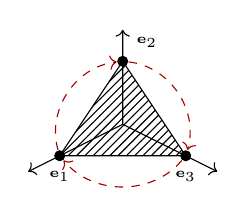
\begin{tikzpicture}[scale=0.8, baseline={(current bounding box.center)}]
        \tikzstyle{point}=[circle,fill,inner sep=0pt, minimum width=4pt, minimum height=4pt]

        % Triangle vertices
        \node[label=above right:\tiny$\bfe_2$] (e3)[point] at (1,1.5) {};
        \node[label=below:\tiny$\bfe_3$] (e1)[point] at (2,0) {};
        \node[label=below:\tiny$\bfe_1$] (e2)[point] at (0,0) {};

        % Barycenter
        \coordinate (bary) at (1,0.5) {}; 

        % Draw the triangle
        \draw[pattern=north east lines] (e1.center) -- (e2.center) -- (e3.center) -- cycle;

        % Compute extended axis endpoints
        \coordinate (e1_ext) at ($(bary) !1.5! (e1)$);
        \coordinate (e2_ext) at ($(bary) !1.5! (e2)$);
        \coordinate (e3_ext) at ($(bary) !1.5! (e3)$);

        % Draw coordinate axes
        \draw[->] (bary.center) -- (e1_ext);
        \draw[->] (bary.center) -- (e2_ext);
        \draw[->] (bary.center) -- (e3_ext);

        % Curved arrows showing clockwise direction around the triangle
        \draw[darkcandyapplered, dashed, ->, bend left=50] (e1) to (e2);
        \draw[darkcandyapplered, dashed, ->, bend left=50] (e2) to (e3);
        \draw[darkcandyapplered, dashed, ->, bend left=50] (e3) to (e1);
    \end{tikzpicture}
}

\newcommand{\triangleWithRotationn}{%
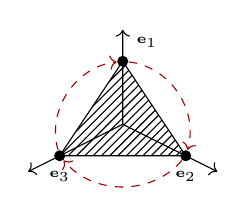
\begin{tikzpicture}[scale=0.8, baseline={(current bounding box.center)}]
        \tikzstyle{point}=[circle,fill,inner sep=0pt, minimum width=4pt, minimum height=4pt]

        % Triangle vertices
        \node[label=above right:\tiny$\bfe_1$] (e3)[point] at (1,1.5) {};
        \node[label=below:\tiny$\bfe_2$] (e1)[point] at (2,0) {};
        \node[label=below:\tiny$\bfe_3$] (e2)[point] at (0,0) {};

        % Barycenter
        \coordinate (bary) at (1,0.5) {}; 

        % Draw the triangle
        \draw[pattern=north east lines] (e1.center) -- (e2.center) -- (e3.center) -- cycle;

        % Compute extended axis endpoints
        \coordinate (e1_ext) at ($(bary) !1.5! (e1)$);
        \coordinate (e2_ext) at ($(bary) !1.5! (e2)$);
        \coordinate (e3_ext) at ($(bary) !1.5! (e3)$);

        % Draw coordinate axes
        \draw[->] (bary.center) -- (e1_ext);
        \draw[->] (bary.center) -- (e2_ext);
        \draw[->] (bary.center) -- (e3_ext);

        % Curved arrows showing clockwise direction around the triangle
        \draw[darkcandyapplered, dashed, ->, bend left=50] (e1) to (e2);
        \draw[darkcandyapplered, dashed, ->, bend left=50] (e2) to (e3);
        \draw[darkcandyapplered, dashed, ->, bend left=50] (e3) to (e1);
    \end{tikzpicture}
}

\newcommand{\triangleWithReflection}{%
    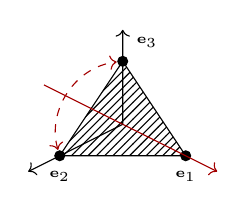
\begin{tikzpicture}[scale=0.8, baseline={(current bounding box.center)}]
        \tikzstyle{point}=[circle,fill,inner sep=0pt, minimum width=4pt, minimum height=4pt]

        % Triangle vertices
        \node[label=above right:\tiny$\bfe_3$] (e3)[point] at (1,1.5) {};
        \node[label=below:\tiny$\bfe_1$] (e1)[point] at (2,0) {};
        \node[label=below:\tiny$\bfe_2$] (e2)[point] at (0,0) {};

        % Barycenter
        \coordinate (bary) at (1,0.5) {}; 

        % Draw the triangle
        \draw[pattern=north east lines] (e1.center) -- (e2.center) -- (e3.center) -- cycle;

        % Compute extended axis endpoints
        \coordinate (e1_ext) at ($(bary) !1.5! (e1)$);
        \coordinate (e2_ext) at ($(bary) !1.5! (e2)$);
        \coordinate (e3_ext) at ($(bary) !1.5! (e3)$);

        % Draw coordinate axes
        \draw[darkcandyapplered,->] (bary.center) -- (e1_ext);
        \draw[->] (bary.center) -- (e2_ext);
        \draw[->] (bary.center) -- (e3_ext);

        % Make the e1 axis red and extend it beyond the midpoint of e2-e3
        \coordinate (mid_e2_e3) at ($(e2)!0.5!(e3)$); % Midpoint of e2 and e3
        \coordinate (e1_extended) at ($(e1)!1.5!(mid_e2_e3)$); % Extend e1 axis beyond midpoint
        \draw[darkcandyapplered] (bary.center) -- (e1_extended); % Red e1 axis extended
        
        \draw[darkcandyapplered, dashed, <->, bend left=50] (e2) to (e3);
    \end{tikzpicture}
}

\newcommand{\triangleWithReflectionn}{%
    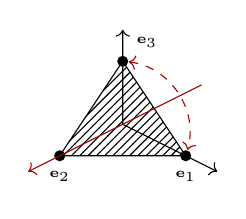
\begin{tikzpicture}[scale=0.8, baseline={(current bounding box.center)}]
        \tikzstyle{point}=[circle,fill,inner sep=0pt, minimum width=4pt, minimum height=4pt]

        % Triangle vertices
        \node[label=above right:\tiny$\bfe_3$] (e3)[point] at (1,1.5) {};
        \node[label=below:\tiny$\bfe_1$] (e1)[point] at (2,0) {};
        \node[label=below:\tiny$\bfe_2$] (e2)[point] at (0,0) {};

        % Barycenter
        \coordinate (bary) at (1,0.5) {}; 

        % Draw the triangle
        \draw[pattern=north east lines] (e1.center) -- (e2.center) -- (e3.center) -- cycle;

        % Compute extended axis endpoints
        \coordinate (e1_ext) at ($(bary) !1.5! (e1)$);
        \coordinate (e2_ext) at ($(bary) !1.5! (e2)$);
        \coordinate (e3_ext) at ($(bary) !1.5! (e3)$);

        % Draw coordinate axes
        \draw[->] (bary.center) -- (e1_ext);
        \draw[darkcandyapplered,->] (bary.center) -- (e2_ext);
        \draw[->] (bary.center) -- (e3_ext);

        % Make the e2 axis red and extend it beyond the midpoint of e1-e3
        \coordinate (mid_e1_e3) at ($(e1)!0.5!(e3)$); % Midpoint of e1 and e3
        \coordinate (e2_extended) at ($(e2)!1.5!(mid_e1_e3)$); % Extend e2 axis beyond midpoint
        \draw[darkcandyapplered] (bary.center) -- (e2_extended); % Red e2 axis extended

        % Curved clockwise arrows for the other axes
        \draw[darkcandyapplered, dashed, <->, bend left=50] (e3) to (e1);
    \end{tikzpicture}
}

\newcommand{\triangleWithReflectionnn}{%
    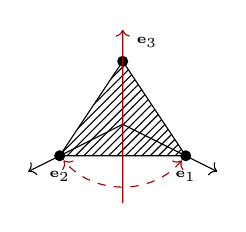
\begin{tikzpicture}[scale=0.8, baseline={(current bounding box.center)}]
        \tikzstyle{point}=[circle,fill,inner sep=0pt, minimum width=4pt, minimum height=4pt]

        % Triangle vertices
        \node[label=above right:\tiny$\bfe_3$] (e3)[point] at (1,1.5) {};
        \node[label=below:\tiny$\bfe_1$] (e1)[point] at (2,0) {};
        \node[label=below:\tiny$\bfe_2$] (e2)[point] at (0,0) {};

        % Barycenter
        \coordinate (bary) at (1,0.5) {}; 

        % Draw the triangle
        \draw[pattern=north east lines] (e1.center) -- (e2.center) -- (e3.center) -- cycle;

        % Compute extended axis endpoints
        \coordinate (e1_ext) at ($(bary) !1.5! (e1)$);
        \coordinate (e2_ext) at ($(bary) !1.5! (e2)$);
        \coordinate (e3_ext) at ($(bary) !1.5! (e3)$);

        % Draw coordinate axes
        \draw[->] (bary.center) -- (e1_ext);
        \draw[->] (bary.center) -- (e2_ext);
        \draw[darkcandyapplered,->] (bary.center) -- (e3_ext);

        % Make the e3 axis red and extend it beyond the midpoint of e1-e2
        \coordinate (mid_e1_e2) at ($(e1)!0.5!(e2)$); % Midpoint of e1 and e2
        \coordinate (e3_extended) at ($(e3)!1.5!(mid_e1_e2)$); % Extend e3 axis beyond midpoint
        \draw[darkcandyapplered] (bary.center) -- (e3_extended); % Red e3 axis extended

        % Curved clockwise arrows for the other axes
        \draw[darkcandyapplered, dashed, <->, bend left=50] (e1) to (e2);
    \end{tikzpicture}
}

% Start matrix with increased spacing
\matrix[column sep=2.5cm, row sep=.5cm] {
    % First row
    \node (T11) {\triangleWithAxes}; & \node (T12) {\triangleWithRotation}; & \node (T13) {\triangleWithRotationn}; \\
    % Second row
    \node (T21) {\triangleWithReflectionnn}; & \node (T22) {\triangleWithReflectionn}; & \node (T23) {\triangleWithReflection}; \\
};

% Add matrices with better spacing to avoid overlap
\node[left=0.2cm of T11] {$\begin{pmatrix} 1 & 0 & 0 \\ 0 & 1 & 0 \\ 0 & 0 & 1 \end{pmatrix}$};
\node[right=0.5cm of T11] {$\begin{pmatrix} 0 & 0 & 1 \\ 1 & 0 & 0 \\ 0 & 1 & 0 \end{pmatrix}$};
\node[right=0.5cm of T12] {$\begin{pmatrix} 0 & 1 & 0 \\ 0 & 0 & 1 \\ 1 & 0 & 0 \end{pmatrix}$};

\node[left=0.2cm of T21] {$\begin{pmatrix} 0 & 1 & 0 \\ 1 & 0 & 0 \\ 0 & 0 & 1 \end{pmatrix}$};
\node[right=0.5cm of T21] {$\begin{pmatrix} 0 & 0 & 1 \\ 0 & 1 & 0 \\ 1 & 0 & 0 \end{pmatrix}$};
\node[right=0.5cm of T22] {$\begin{pmatrix} 1 & 0 & 0 \\ 0 & 0 & 1 \\ 0 & 1 & 0 \end{pmatrix}$};

\node[above= 0.1cm of T11] {\text{Ταυτοτικός}};
\node[above= 0.1cm of T12] {\text{Στροφή κατά $120^\circ$}};
\node[above= 0.1cm of T13] {\text{Στροφή κατά $240^\circ$}};
\node[above= 0.001cm of T21] {\text{Ανάκλαση ως προς $x_3=0$}};
\node[above= 0.001cm of T22] {\text{$x_2=0$}};
\node[above= 0.001cm of T23] {\text{και $x_1=0$}};

\end{tikzpicture}
\]

Το σύνολο αυτών των έξι μετασχηματισμών αποτελεί ομάδα με πράξη τη σύνθεση (γιατί;), η οποία ονομάζεται \defn{ομάδα συμμετρίας} του $\Delta$. Οι ομάδες συμμετρίας τριγώνων μεγαλύτερης διάστασης θα είναι οι πρωταγωνιστές αυτού του μαθήματος.

\begin{definition}
    \label{def:symmetricGroup}
    Έστω $S$ ένα σύνολο. \defn{Μετάθεση} του $S$ ονομάζεται κάθε αμφιμονοσήμαντη απεικόνιση $S \to S$. Το σύνολο $\fS(S)$ όλων των μεταθέσεων του $S$ με πράξη την σύνθεση απεικονίσεων αποτελεί ομάδα, η οποία ονομάζεται \defn{συμμετρική ομάδα} του $S$. Στην περίπτωση όπου $S$ είναι το σύνολο\footnote{Το σύμβολο $\coloneqq$ σημαίνει \textquote{εξ' ορισμού}.} $[n] \coloneqq \{1, 2, \dots, n\}$, τότε γράφουμε $\fS_n$.
\end{definition}

Μια μετάθεση $\pi \in \fS_n$ συνήθως γράφεται στην μορφή
\[
\begin{pmatrix}
    1     & 2     & \cdots & n \\
    \pi_1 & \pi_2 & \cdots & \pi_n
\end{pmatrix}
\]
όπου $\pi_i \coloneqq \pi(i)$, για κάθε $i \in [n]$, ή ως \emph{λέξη}
\[
\pi_1\pi_2\cdots\pi_n,
\]
ή στην \emph{κυκλική μορφή} ως γινόμενο ξένων κύκλων. Για παράδειγμα, 
\[
\pi \ = \ 
\begin{pmatrix}
    1 & 2 & 3 & 4 & 5 & 6 \\
    3 & 4 & 1 & 6 & 5 & 2
\end{pmatrix}
\ = \
341652
\ = \
\cycle{1,3}\cycle{2,4,6}\cycle{5} \ \in \fS_6.
\] 

Θα δούμε περισσότερα για τις μεταθέσεις και την συμμετρική ομάδα σε επόμενες παραγράφους. Οι μεταθέσεις μπορούν να \textquote{αναπαρασταθούν} με πολλούς διαφορετικούς τρόπους κι αυτό τις καθιστά ένα πολύ πλούσιο αντικείμενο μελέτης στην \emph{αλγεβρική συνδυαστική}. 

Ένα από τα στοιχεία που κάνουν τις ομάδες ενδιαφέρουσες είναι ότι δρουν σε διάφορα μαθηματικά αντικείμενα.

\begin{definition}
    \label{def:groupAction}
    Έστω $G$ μια ομάδα με ουδέτερο στοιχείο $\epsilon$ και $S$ ένα σύνολο. \defn{Δράση} της $G$ πάνω στο $S$ ονομάζεται μια απεικόνιση\footnote{Όπως και με την πράξη της ομάδας, έτσι και εδώ, συχνά θα παραλείπουμε το σύμβολο $\cdot$.} $\cdot : G \times S \to S$ τέτοια ώστε 
    %
    \begin{itemize}
        \item $g \cdot (h \cdot s) = (gh) \cdot s$
        \item $\epsilon \cdot s = s$
    \end{itemize}
    %
    για κάθε $g, h \in G$ και $s \in S$. Στην περίπτωση αυτή το $S$ ονομάζεται \defn{$G$-σύνολο}.
\end{definition}

Αν $S$ είναι ένα $G$-σύνολο, τότε η δράση κάθε στοιχείου $g \in G$ στο $S$ μεταθέτει τα στοιχεία του. Πιο συγκεκριμένα, η απεικόνιση 
\begin{align*}
    \sigma_g: S &\to S \\
    s &\mapsto gs
\end{align*}
είναι αμφιμονοσήμαντη (γιατί;).

Ένα $G$-σύνολο επάγει μια \emph{διαμέριση} της $S$ \emph{ταυτίζοντας} όλα εκείνα τα στοιχεία του $S$ τα οποία μπορούν να προκύψουν έπειτα από διαδοχικές εφαρμογές στοιχείων της $G$. Κάθε τέτοιο υποσύνολο του $S$
\[
\oO_s \coloneqq \{gs : g \in G\}
\] 
ονομάζεται \defn{τροχιά} του $s$. Αν η ομάδα $G$ είναι πεπερασμένη, τότε 
%
\begin{equation}
    \label{eq:counting_formula}
    \abs{\oO_s} = \frac{\abs{G}}{\abs{G_s}},
\end{equation}
%
όπου $G_s$ είναι το σύνολο όλων των $g \in G$ τα οποία \emph{σταθεροποιούν} το $s$, δηλαδή $gs = s$ (γιατί;).

Για παράδειγμα, η συμμετρική ομάδα $\fS_n$ δρα στο $[n]$ με τον προφανή τρόπο:
\[
\pi \cdot i \coloneqq \pi_i.
\]
Η δράση αυτή έχει μόνο \emph{μια} τροχιά και κατά συνέπεια $\abs{\oO_i} = n$, για κάθε $i \in [n]$. Τέτοιες δράσεις ονομάζονται \defn{μεταβατικές}. Η Ταυτότητα~\eqref{eq:counting_formula} μας πληροφορεί ότι 
\[
\abs{\left(\fS_n\right)_i} = (n-1)!,
\]
για κάθε $i \in [n]$. Πράγματι, ο σταθεροποιητής οποιουδήποτε στοιχείου του $[n]$ είναι ένα \textquote{αντίγραφο} της $\fS_{n-1}$ (γιατί;). 

Δεν είναι όμως όλες οι δράσεις μεταβατικές. Για παράδειγμα, για $n = 5$, θεωρούμε την υποομάδα της $\fS_5$ που παράγεται από τις αντιμεταθέσεις $\cycle{1,3}$ και $\cycle{2,5}$. Η δράση αυτή έχει 3 τροχιές (γιατί;) και η επαγόμενη διαμέριση είναι\footnote{Το σύμβολο $\uplus$ σημαίνει ξένη ένωση.} 
\[
[5] \ = \ \{1, 3\} \uplus \{4\} \uplus \{2, 5\} .
\]

\begin{example}
    \label{ex:group_actions}
    Έστω $G$ μια ομάδα. Ας δούμε δυο σημαντικά παραδείγματα δράσεων ομάδων.
    \begin{itemize}
        \item[(1)] Έστω $H$ μια υποομάδα της $G$. Για $g \in G$, το σύνολο
        \[
        gH \coloneqq \{gh : h \in H\}
        \]
        ονομάζεται \defn{αριστερό σύμπλοκο} της $H$ στην $G$. 
        Το σύνολο των αριστερών συμπλόκων της $H$ επάγει μια διαμέριση της $G$, δηλαδή 
        \[
        G = t_1H \biguplus t_2H \biguplus \cdots \biguplus t_mH
        \]
        για κάποια\footnote{Το σύνολο $\{t_1, t_2, \dots, t_m\}$ συνήθως ονομάζεται \emph{σύστημα αντιπροσώπων} των αριστερών συμπλόκων της $H$.} $t_1, t_2, \dots, t_m \in G$, με φυσικό τρόπο, ταυτίζοντας δυο αριστερά σύμπλοκα $gH = xH$ αν και μόνο αν $x^{-1}g \in H$.

        Για παράδειγμα, αν $G = \fS_3$ και $H$ είναι η υποομάδα που παράγεται από την μετάθεση $\cycle{2,3}$, τότε έχουμε τη διαμέριση 
        \[
        \fS_3 = H \uplus \cycle{1,2}H \uplus \cycle{1,3}H.
        \]
        Παρατηρούμε ότι $\cycle{1,2}H = \cycle{1,2,3}H$ αφού 
        \[
        \cycle{1,2,3}^{-1}\cycle{1,2} = \cycle{1,3,2}\cycle{1,2} = \cycle{2,3} \ \in H.
        \]
        Ομοίως για το $\cycle{1,3}H = \cycle{1,3,2}H$.

        H $G$ δρα (μεταβατικά) στο σύνολο των αριστερών συμπλόκων της $H$ θέτοντας
        \[
        x \cdot gH = xgH,
        \]
        για κάθε $x ,g \in G$. Στην περίπτωση όπου $H = \{\epsilon\}$ είναι η τετριμμένη υποομάδα, τότε η $G$ δρα στον εαυτό της με \defn{αριστερό πολλαπλασιασμό}.

        \item[(2)] Η $G$ δρα στον εαυτό της με \defn{συζυγία}, θέτοντας
        \[
        g \cdot x = gxg^{-1}
        \]
        για κάθε $x, g \in G$. Οι τροχιές αυτής της δράσης ονομάζονται \defn{κλάσεις συζυγίας}. Δυο στοιχεία $t, x \in G$ που ανήκουν στην ίδια τροχιά, δηλαδή αν $x = gtg^{-1}$, για κάποιο $g \in G$ ονομάζονται \defn{συζυγή}. 

        Στην περίπτωση όπου η $G$ είναι πεπερασμένη, το πλήθος των στοιχείων μιας κλάσης συζυγίας μπορεί να υπολογιστεί από την Ταυτότητα~\eqref{eq:counting_formula}. Το να έχει μια κλάση συζυγίας ένα μόνο στοιχείο $x$ σημαίνει ότι $x = gxg^{-1}$, \emph{για κάθε} $g \in G$. Το σύνολο όλων των στοιχείων της $G$ με αυτή την ιδιότητα ονομάζεται \defn{κέντρο} της $G$ και συμβολίζεται με $\rmZ(G)$.

        Για παράδειγμα, η συμμετρική ομάδα $\fS_3$ έχει τρεις κλάσεις συζυγίας: 
        \[
        \fS_3 = \{\cycle{1,2,3}\} \uplus \{\cycle{1,2}, \cycle{2,3}, \cycle{1,3}\} \uplus \{\cycle{1,2,3}, \cycle{1,3,2}\}.
        \]
        Αργότερα, θα μελετήσουμε με περισσότερη λεπτομέρεια τις κλάσεις συζυγίας της συμμετρικής ομάδας.
    \end{itemize}
\end{example}

Στην περίπτωση όπου έχουμε ένα $G$-σύνολο $S$, μπορούμε να \textquote{αναπαραστήσουμε} την $G$ ως υποομάδα της ομάδας συμμετρίας του $S$. Πιο συγκεκριμένα, η απεικόνιση 
\begin{align*}
    \sigma : G &\to \fS(S) \\
    g &\mapsto \sigma_g
\end{align*}
είναι \emph{ομομορφισμός ομάδων}, δηλαδή ικανοποιεί τις σχέσεις:
\begin{align*}
    \sigma(\epsilon) &= \rmid_S \\ 
    \sigma(gx) &= \sigma_g\sigma_x
\end{align*}
για κάθε $g, x \in G$, οπου $\rmid_S$ είναι η ταυτοτική απεικόνιση του $S$ (γιατί;).

Πίσω στο παράδειγμα του τριγώνου $\Delta$, η συμμετρική ομάδα $\fS_3$ δρα στον $\RR^3$, και κατά συνέπεια στο $\Delta$, μεταθέτοντας τα στοιχεία της βάσης του (δηλαδή, τις κορυφές του $\Delta$):
\[
w\cdot \bfe_i \coloneqq \bfe_{w_i},
\] 
για κάθε $w\in \fS_3$ και $1 \le i \le 3$. Κάθε $w \in \fS_3$ επάγει μια διαφορετική\footnote{Οι δράσεις με αυτή την ιδιότητα ονομάζονται \defn{πιστές}.} μετάθεση $\sigma(w)$ (γιατί;). Συνεπώς, η $\sigma$ είναι \textquote{πιστή αναπαράσταση} της $\fS_3$ στην ομάδα συμμετρίας του τριγώνου, η οποίες είναι \emph{ισόμορφες}.

Στην περίπτωση αυτή, το σύνολο $\RR^3$ έχει την έξτρα δομή του \emph{διανυσματικού χώρου} και κάθε μετάθεση $\sigma(w)$ είναι \emph{γραμμικός μετασχηματισμός}. Υπολογίζοντας του πίνακες ως προς τη συνήθη βάση $\{\bfe_1, \bfe_2, \bfe_3\}$ βρίσκουμε 
\[
\begin{array}{ccc}
    \sigma(123) = 
    \begin{pmatrix} 
        1 & 0 & 0 \\ 
        0 & 1 & 0 \\ 
        0 & 0 & 1 
    \end{pmatrix}  
    & \sigma(231) = 
    \begin{pmatrix} 
        0 & 0 & 1 \\ 
        1 & 0 & 0 \\ 
        0 & 1 & 0 
    \end{pmatrix}
    & \sigma(312) = 
    \begin{pmatrix} 
        0 & 1 & 0 \\ 
        0 & 0 & 1 \\ 
        1 & 0 & 0 
    \end{pmatrix} \\
     &  &  \\
    \sigma(213) =
    \begin{pmatrix} 
        0 & 1 & 0 \\ 
        1 & 0 & 0 \\ 
        0 & 0 & 1 
    \end{pmatrix} 
    & \sigma(321) = 
    \begin{pmatrix} 
        0 & 0 & 1 \\ 
        0 & 1 & 0 \\ 
        1 & 0 & 0 
    \end{pmatrix} 
    & \sigma(132) = 
    \begin{pmatrix} 
        1 & 0 & 0 \\ 
        0 & 0 & 1 \\ 
        0 & 1 & 0 
    \end{pmatrix}.
\end{array}
\]
Οι μετασχηματισμοί αυτοί λοιπόν είναι οι συμμετρίες του $\Delta$ που συναντήσαμε νωρίτερα! Αυτή είναι και η βασική ιδέα της αναπαράστασης μιας ομάδας.

\begin{definition}
    \label{def:representation}
    Έστω $G$ μια ομάδα. \defn{Αναπαράσταση} της $G$ ονομάζεται ένα ζεύγος $(\rho, V)$, όπου 
    \begin{itemize}
    \item $V$ είναι διανυσματικός χώρος 
    \item $\rho : G \to \GL(V)$ είναι ένας ομομορφισμός ομάδων, 
    \end{itemize}
    όπου με $\GL(V)$ συμβολίζουμε την ομάδα των αντιστρέψιμων γραμμικών μετασχηματισμών του $V$\footnote{Αυτή ονομάζεται \defn{γενική γραμμική} ομάδα του $V$.}. Η διάσταση του $V$ ονομάζεται \defn{διάσταση} (ή \defn{βαθμός}) της αναπαράστασης.
\end{definition}

Με άλλα λόγια, αναπαράσταση της $G$ είναι ένα $G$-σύνολο $V$ με δομή διανυσματικού χώρου, την οποία \textquote{σέβεται} η δράση. Συχνά, αντί για $\rho(g)(v)$ θα γράφουμε απλώς $g \cdot v$, ή ακόμα πιο απλά $gv$. Στην περίπτωση αυτή θα λέμε ότι το $V$ είναι ένα \defn{$G$-πρότυπο}. Επίσης, όταν ο $V$ έχει πεπερασμένη διάσταση (που είναι και η περίπτωση ενδιαφέροντος για αυτό το μάθημα), τότε διαλέγοντας μια βάση του $V$ μπορούμε να αναπαραστήσουμε το $\rho(g)$ ως ένα αντιστρέψιμο πίνακα. Σε ότι ακολουθεί, θα εναλλάσσουμε μεταξύ πινάκων και γραμμικών μετασχηματισμών χωρίς να το αναφέρουμε, αλλά θα είναι κατανοητό από τα συμφραζόμενα.

Τι γίνεται όμως αν έχουμε μια δράση σ' ένα σύνολο που δεν έχει (απαραίτητα) τη δομή διανυσματικού χώρου? Κάθε δράση ομάδας επάγει μια αναπαράσταση ως εξής. Έστω $S = \{s_1, s_2, \dots, s_n\}$ ένα $G$-σύνολο και $\FF[S]$ ο διανυσματικός χώρος που παράγεται από το $S$\footnote{Στην πράξη θα γράφουμε $\FF[s_1, s_2, \dots, s_n]$ \textquote{ξεχνώντας} τις αγκύλες και θα αναφερόμαστε στο $S$ ως  τη \defn{συνήθη βάση} του χώρου αυτού.}. Επεκτείνουμε γραμμικά την δράση στο $\FF[S]$ θέτοντας 
\[
g\left(c_1s_1 + c_2s_2 + \cdots + c_ns_n\right) \ \coloneqq
c_1 gs_1 + c_2 gs_2 + \cdots + c_n gs_n
\] 
για κάθε $g \in G$ και $c_1, c_2, \dots, c_n \in \FF$, δίνοντας έτσι στο $\FF[S]$ την δομή $G$-προτύπου.

Η αντίστοιχη αναπαράσταση ονομάζεται \defn{αναπαράσταση μεταθέσεων} (permutation representation). Τέτοιου είδους αναπαραστάσεις είναι πολύ σημαντικές, διότι μας επιτρέπουν να χρησιμοποιούμε μεθόδους συνδυαστικής για να μελετήσουμε την ομάδα.
\end{document}